\chapter{Experiments}
\label{ch.experiments}

% Neste capítulo
	Neste capítulo é avaliado o performance da troca de dados dos serviços do Nanvix Microkernel no MPPA, ie, mailbox e portal.
	Os benchmarks buscam estimular diversas configurações de comunicação coletiva que são comuns em um sistema distribuído.
	% Especificamente, eles examinaram o lado receptor para evidenciar o impacto dos serviços 
	Especificamente, configurações que estaram presentes nos serviços de alto nível exportados pelo Nanvix Multikernel.
	Por exemplo, a troca de mensagens entre servidores e clientes, distribuição de trabalho, e a coleta dos resultados da distribuição.
	Apesar do serviço Sync não possuir experimentos específicos, ele foi utilizado em todos os benchmarks para sincronizar todos os nós antes de iniciarem as comunicações.

% Como foram medidos os dados
	Os dados foram coletados através da interface IOCTL de cada serviço.
	Deste modo, os dados mensurados representam efetivamente a comunicação, amenizando o impacto da configuração do benchmark.
% Quais as configurações do mppa
	Em cada cluster foi utilizado apenas 1 PE para rodar a aplicação.
	Este PE solicitou os serviços do Microkernel para performar a comunicação.
	Todos os benchmarks consideram 1 cluster I/O e 16 clusters de computação.
	No clusters I/O foi utilizado apenas uma das interfaces disponíveis por causa da limitação do envio ser realizado explicitamente pelo núcleo mestre.
	Quando a rotina de comunicação necessitar de um nó mestre, o cluster I/O assume este papel.

% Quantas iterações, limitações de memória e desvio padrão
	O MPPA apresenta características intrínsecas que garantem uma baixa variabilidade entre as execuções.
	Deste modo, foram realizados 50 iterações de cada benchmarks.
	As 10 primeiras foram descartadas para eliminar o período de aquecimento.
	Nos testes do serviço Portal, as quantidades de dados transferidos seguem um ordem exponencial.
	Entretanto, a restrição de memória interna nos Cluster de computação limitou a quantidade de transferencia a 64 KB.
	Por fim, todos os resultados mostraram um erro padrão menor que 1\%.

	\section{Micro-benchmarks}

		Para analise da performance dos Serviços de Comunicação foram utilizados as rotinas típicas para comunicação coletiva do MPI e comportamentos comuns entre clientes e servidores.
		As subseções a seguir introduziram conceitualmente cada uma dessas rotinas.

		\subsection{Broadcast}

			Broadcast é a técnica mais comum dentre as rotinas de comunicação coletiva do MPI.
			Nesta rotina, um nó envia o mesmo dado para todos os nós existentes.
			Este envio pode ser implementado de diversas formas.
			Por exemplo, flat tree, binary tree, double tree e chain~\cite{survey-mpi}.
			A Figura (broadcast) apresenta o algoritmo flat tree utilizado no benchmark.
			A flat tree define que o nó raiz deve enviar o dado para todos mundo, sem delegar esta função a outros nós. 
			Esta rotina pode ser utilizada para enviar inputs do usuário a um programa paralelo, ou enviar parametros de configuração para todos os nó~\cite{url:mpitutorial}.

			\begin{figure}[!tb]
				\centering%
				\caption{Example of \mpi Broadcast}%
				\label{fig:exp-broadcast}%
				\includegraphics[width=.6\textwidth]{mpi-broadcast.pdf}%
				\fonte{Adapted from \citeonline{url:mpitutorial}.}%
			\end{figure}

		% \subsection{Scatter}

		% 	\begin{figure}[!tb]
		% 		\centering%
		% 		\caption{Example of \mpi Scatter}%
		% 		\label{fig:mpi-scatter}%
		% 		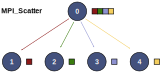
\includegraphics[width=.6\textwidth]{mpi-scatter.pdf}%
		% 		\fonte{Adapted from \citeonline{url:mpitutorial}.}%
		% 	\end{figure}

		% 	In this benchmark, I will write about ...

		\subsection{Gather}

			Gather é a operação inversa de uma variante do broadcast, chamada scatter.
			A Figura (gather) ilustra o fluxo inverso de dados, onde esta rotina reúne os  dados distribuídos em um único nó~\cite{url:mpitutorial}.
			De forma análoga ao broadcast, foi implementado uma flat tree onde todos os nós raízes enviam suas partes diretamente ao nó raiz.

			\begin{figure}[!tb]
				\centering%
				\caption{Example of \mpi Gather}%
				\label{fig:exp-gather}%
				\includegraphics[width=.6\textwidth]{mpi-gather.pdf}%
				\fonte{Adapted from \citeonline{url:mpitutorial}.}%
			\end{figure}

		\subsection{AllGather}

			AllGather é uma rotina que não possui um nó raíz, ilustrado pela Figura (allgather).
			Como o nome sugere, a rotina executa diversas operações Gather para que todos os nós participantes terminem com todas as partes dos dados reúnidos.
			Alguns algorítmos possíveis são Ring Algorithm, Recursive Doubling, Gather followed by Broadcast Algorithm.
			O benchmark implementa o Bruck Algorithm onde cada nó enviará seu dado para um nó com distância i e receberá dados de uma distância -i, até que todos os nós contenham o dado completo.

			\begin{figure}[!tb]
				\centering%
				\caption{Example of \mpi AllGather}%
				\label{fig:exp-allgather}%
				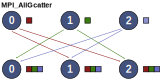
\includegraphics[width=.6\textwidth]{mpi-allgather.pdf}%
				\fonte{Adapted from \citeonline{url:mpitutorial}.}%
			\end{figure}

		\subsection{Ping-Pong}

			Ping-pong não é uma rotina de comunicação coletiva do MPI mas representa a comunicação de um servidor respondendo requisições de nós clientes.
			A Figura (ping-pong) ilustra a comunicação se concentrando no nó mestre, onde o mestre recebe e responde uma requisição de cada vez.

			\begin{figure}[!tb]
			    \centering%
			    \caption{Example of Ping-Pong}%
			    \label{fig:exp-ping-pong}%
			    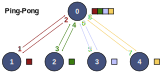
\includegraphics[width=.6\textwidth]{mpi-ping-pong.pdf}%
			    \fonte{Develop by the Author.}%
			\end{figure}

	\section{Throuput}

		In this section, I will write about ...